\chapter{Digital Communication}
This first section is all about how to convert and transmit some signal.\
\begin{section}{Introduction}
The goal of communication is to transmit some kind of data form a sender to a receiver. In order 
to do so, the physical layer defines the means of transmitting a stream of \textbf{raw bits} over a
physical data link, which connects those two nodes.\\
Data is transmitted in the form of \textbf{signals}, which are a physical representation of the data.
The signal is transmitted over a \textbf{channel}, which is the transmission medium that connects 
the sender and receiver. This can be both wired or wireless.\\
Whereas with wired channels, checking the device connected to the channel is easier to implement, 
with wireless ones security is a major when travelling in the channel. This is for may reasons:
\begin{itemize}
  \item No inherent protection is applied to the channel( it is replaced by a logical association)
     \subitem sending and receiving messages do not need physical access to the network 
     infrastructure
  \item the communication is in broadcast, which is intrinsic of radio nature.
    \subitem Transmission can be overheard by anyone in range( which can be quite big, depending 
    on the situation), and anyone can generate a transmission, for example by jamming nearby 
    transmissions.
\end{itemize}
As a result:
\begin{itemize}
  \item Eavesdropping is easy
  \item Injecting fake messages into the communication in easy
  \item replaying previously recorded messages is easy(\textit{meaconing}). This is actually very 
    dangerous for gps positioning, so it is also a security concern.
  \item illegitimate access to the network and its services is easy
  \item Denial of service attacks are easy, achieved by jamming the channel.
\end{itemize}
% 9/43
\end{section}
\begin{section}{Digital Communication System}
The digital communication system in characterized by three sections: 

\begin{itemize}
  \item the \textbf{user section}, which consist in the transmitter and the receiver, that want to 
    communicate. 
  \item the \textbf{interface section}, which is the interface to conveying the signal from the 
    user to the analog channel. It also transforms bits to analog signal, compressing and encoding 
    them, also associating bits to signal waveforms, to transform bits to analog signal.
  \item the \textbf{channel section}, which is the physical medium, that can only propagate analog 
    waveforms. In the end, we want to transmit digital signal but we are forced to use analog ones.
\end{itemize}

\begin{figure}[h]
  \centering
  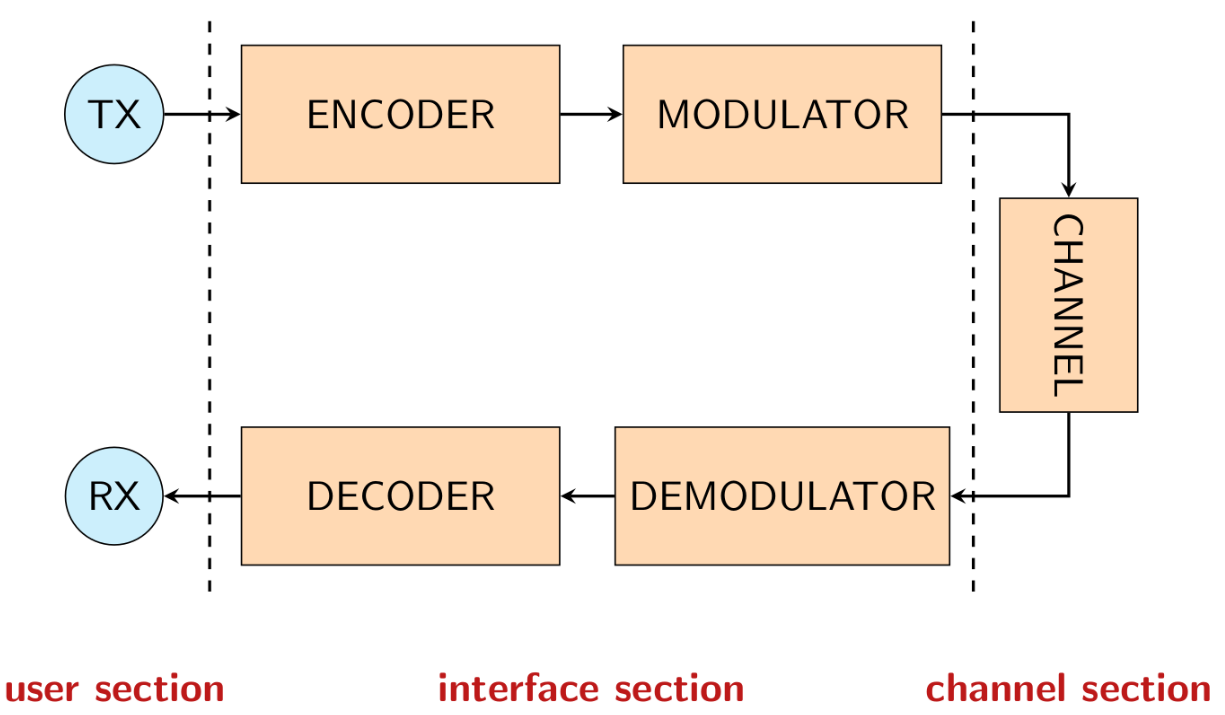
\includegraphics[width=0.7\textwidth]{img/digital communication schema.png}
  \caption{Digital Communication System}
  \label{fig:Digital Communication System}
\end{figure}
\begin{subsection}{The transmitter chain}
The transmitter chain is the part of the system that takes the digital signal, or an analog one 
converted to digital, and converts it to an analog signal, that can be transmitted over the
channel.\\
It is basically composed by two parts. The first one being an \textbf{encoder}, which can limit the amount 
of bits transmitted(\textit{source encoding}), and/or make the transmitted sequence more robust to
errors(\textit{channel encoding}).\\
The second one is the \textbf{modulator}, which is the part of the system that takes the digital
signal and converts it to an analog one to transmit it over the channel.
\end{subsection}
\begin{subsection}{The channel}
The channel is the physical medium that transfers bits from interface to interface, from the sender
to the receiver.
Its operation is affected by different types of disturbances such as:
\begin{itemize}
	\item frequency-domain distortion
	\item wireless fading
	\item additive noise
	\item impulsive noise
	\item interference from other frequency channels (interchannel interference)
	\item interference from the same frequency channel (cochannel interference)
	\item Intentional interference
\end {itemize}
\end{subsection}
\begin{subsection}{The receiver chain}
The receiver chain is the part of the system that takes the analog signal from the channel and
converts it to a digital signal, that can be processed by the user.\\
It is composed by the dual counterpart of the transmitter chain, the \textbf{demodulator} and the
\textbf{decoder}. \\
The demodulator takes the analog signal and converts it to a sequence of samples that can be
processed by the decoder.\\
The decoder takes the sequence of samples and converts it to a digital signal. It implements
\textit{channel decoding}, to correct errors, and \textit{source decoding}, to recover the original
message.
\end{subsection}
\end{section}

\begin{section}{Signal representation and Processing}
  \begin{boxH}
    A \textbf{signal} is a (mathematical) function that conveys information about a phenomenon.
  \end{boxH}
  Basically, any quantity that varies over space or time can be used to represent a informations,
  allowing to describe the evolution of physical quantities over time(voltages, currents, \dots).\\
  Its mathematical representation is therefore a function of real variable (time) taking real or 
  complex(more than one) values.\\
  We will be mostly focused on Electromagnetic Signals (e.g. voltage), but the general concepts 
  can be applied to any kind of signal
  \begin{subsection}{Energy of a signal}
    The energy of a signal is the integral of the squared modulus of the signal itself.
    \begin{equation}
      E(x) = \int_{-\infty}^{\infty} |x(t)|^2 dt
    \end{equation}
    As we can see , the energy is a scalar value, and the whole function is made positive by the
    squared modulus.\\
    \begin{figure}[h]
      \centering
      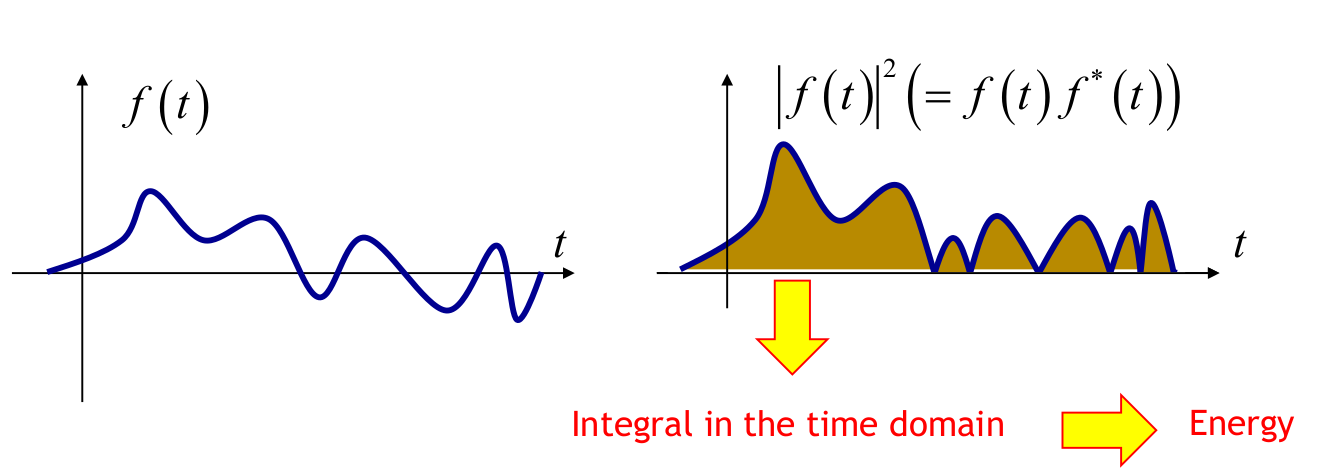
\includegraphics[width=0.7\textwidth]{img/energy signal.png}
      \caption{Energy of a signal}
      \label{fig:Energy of a signal}
    \end{figure}
    A signal with a very large amplitude, over time, will have a very high energy, while a signal
    which assumes values close to zero will have a very low energy, being a very weak signal.\\
    Furthermore, we can note that the more distant is the signal from the origin, the larger the energy.
  \end{subsection}
  \begin{subsection}{Power of a signal}
    When we refer to power we can refer to the \textbf{instantaneous power} of a signal, which is just the 
    square module of a signal
    \begin{equation}
      P(x) = |x(t)|^2
    \end{equation}
    but much more commonly we refer to the average power of a signal, which is the time average of
    the instantaneous power of the whole signal.
    \begin{equation}
      P(x) = \lim_{a \to \infty} \frac{1}{2a} \int_{-a}^{a} |x(t)|^2 dt
    \end{equation}
    This a again a scalar value.
  \end{subsection}
  \begin{subsection}{Signal Representation}
    To analyze and process the signals, it is necessary to adequately represent them, and the
    definition of signals as "time functions" is NOT effective for many applications, for many 
    reasons.\\
    Generally, signals can become very complicated depending on our communication system, and
    we want different ways of representing them, to make them easier to process.\\
    For instance, we can represent a signal as a sum of elementary signals, thanks to the scalar
    product of the signal with a basis of the space of signals.\\

    The scalar product between signals is a scalar value, which is a measure of the similarity 
    among signals.\\
    If two function are quite similar we will get a large number.
    It it is zero, they are said to be orthogonal.
    \begin{equation}
      \langle x,y \rangle = \langle x(t),y(t) \rangle = \int_{-\infty}^{\infty} x(t)y^*(t) dt
    \end{equation}

    So, if we have a set of elementary signals $w_1(t), w_2(t), \dots, w_m(t)$, we write the signal
    $x(t)$ as a linear combination of the elementary signals:
    \begin{equation}
      x(t) = \sum_{i=1}^{m} \alpha_i w_i(t)
    \end{equation}
    where $\alpha_i$ are the coefficients of the linear combination $\alpha_i = \langle x(t), 
    w_i(t) \rangle$.\\
    In a more down to hearth way, the coefficient $\alpha_i$ allows us to understand how much each
    individual signal is similar to any other elementary signal we are considering, and because the 
    scalar product is higher for similar signals, we can understand how much each elementary signal
    is contributing to the whole signal.\\

    Furthermore, by adjusting the coefficient, we are able to create a whole different signal using
    the same elementary signals.
    \begin{subsubsection}{A common example: In Phase and Quadrature Representation}
      Lets consider a very simple basis, or a set of elementary signals, which is actually more 
      important that many other ones:
      \begin{itemize}
        \item the \textbf{in-phase} signal, which is a cosine function $w_1(t) = cos(2\pi f_o t)$
        \item the \textbf{quadrature} signal, which is a sine function $w_2(t) = sin(2\pi f_o t)$
      \end{itemize}
      where $f_o$ is the frequency, in Hz, of the signal.\\
      We can write any signal as a linear combination of these two signals, just by adjusting the
      coefficients:
      \begin{equation}
        x(t) = x_1 cos(2\pi f_o t) + x_2 sin(2\pi f_o t)
      \end{equation}
      where x(t) is the signal we want to represent, and $x_1$ and $x_2$ are the coefficients of the
      linear combination.\\

      A very simple representation of this complex signal is obtainable by representing each signal 
      as an axes in a complex plane, for example in figure \ref{fig:Complex Plane} the x-axis 
      is the in-phase signal, and the y-axis is the quadrature signal.\\
      Each signal can be represented as a point in the complex plane, because the distance from the
      origin signal(\textit{axis}) is the amplitude of the signal.
      For example, choosing a point close to the x-axis, we are choosing a signal with a very low
      quadrature component, and a very high in-phase component.\\
      \begin{figure}[h]
        \centering
        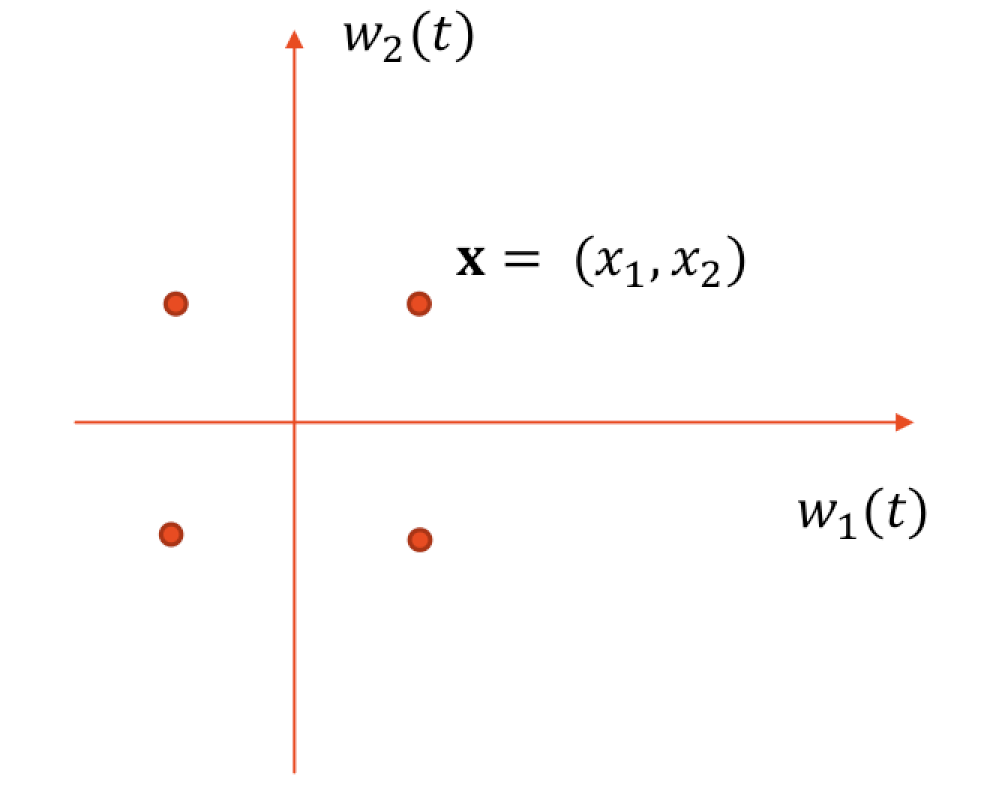
\includegraphics[width=0.5\textwidth]{img/iq representation.png}
        \caption{Some points that represent some signals in the I/Q representation}
        \label{fig:Complex Plane}
      \end{figure}
    \end{subsubsection}
  \end{subsection}
  \begin{subsection}{Fourier Analysis}
    Lets consider a signal with bases the complex exponential functions 
    \begin{equation}
      e^{j2\pi \frac{n}{T} t} = cos(2\pi \frac{n}{T} t) + j sin(2\pi \frac{n}{T} t)
    \end{equation}
    It is actually characterized by a frequency $f_n = \frac{n}{T}$, where T is the period of the
    signal. The higher the frequency, the more oscillations we will have in the same time interval.\\

    We can use that function as a basis to decompose a signal, again.
  \end{subsection}

\end{section}
